\documentclass[9pt,twocolumn]{opticajnl}
\journal{opticajournal}
\setboolean{shortarticle}{true}
% Load siunitx when available; otherwise provide minimal fallbacks so local builds succeed
\newif\ifhavesi
\IfFileExists{siunitx.sty}{\havesitrue}{\havesifalse}
\ifhavesi
  \usepackage{siunitx}
  \sisetup{range-phrase = --, range-units = single}
  \sisetup{per-mode = symbol}
  \DeclareSIUnit{\pixel}{px}
  \DeclareSIUnit{\USD}{USD}
\else
  \newcommand{\sisetup}[1]{}
  \newcommand{\SI}[2]{#1\,#2}
  \newcommand{\SIrange}[3]{#1--#2\,#3}
  \newcommand{\DeclareSIUnit}[2]{}
  % Common unit symbols used in this manuscript
  \providecommand{\nano}{n}
  \providecommand{\micro}{\ensuremath{\mu}}
  \providecommand{\milli}{m}
  \providecommand{\kilo}{k}
  \providecommand{\mega}{M}
  \providecommand{\giga}{G}
  \providecommand{\second}{s}
  \providecommand{\meter}{m}
  \providecommand{\pixel}{px}
  \providecommand{\byte}{B}
  \providecommand{\per}{/}
  \providecommand{\USD}{USD}
\fi
\usepackage{ifthen}
\usepackage{placeins}
\usepackage{xcolor}
\usepackage{tikz}
\usetikzlibrary{arrows.meta,positioning,shadings,calc}
% Outline for high-contrast text over images
\usepackage[outline]{contour}
\contourlength{0.6pt}
% Colors used in event cloud legends
\definecolor{evtPos}{HTML}{FFBB78} % +1 polarity (orange)
\definecolor{evtNeg}{HTML}{AEC7E8} % -1 polarity (blue)

% Yellow placeholder figure macro for drafts
\newcommand{\phfig}[2][0.95\linewidth]{%
  \begingroup\setlength{\fboxsep}{0pt}\colorbox{yellow!20}{%
    \parbox{#1}{\vspace{16mm}\centering\textbf{PLACEHOLDER}\\\small #2\vspace{14mm}}}%
  \endgroup}

\providecommand{\nocitefullrefs}[1]{}

% \title{Self-synchronized event-driven transmission hyperspectral imaging with multi-window scanning compensation}
\title{Self-Calibrated Neuromorphic Hyperspectral Sensing}
% % \author{Author One\authormark{1} and Author Two\authormark{2,*}}
% \author[]{Rongzhou Chen}
% \author[]{Chutian Wang}
% \author[]{Yuqing Cao}
% \author[*]{Edmund Y. Lam}
% \affil[]{Department of Electrical and Electronic Engineering, The University of Hong Kong, Pokfulam, Hong Kong, China}
% % \address{Department of Electrical and Electronic Engineering, The University of Hong Kong, Pokfulam, Hong Kong, China}
% \affil[*]{elam@eee.hku.hk}
\author{Rongzhou Chen, Chutian Wang, Yuqing Cao and Edmund Y. Lam{*}}
\affil{Department of Electrical and Electronic Engineering, The University of Hong Kong, Pokfulam, Hong Kong SAR, China}
% \affil[*]{elam@eee.hku.hk}
\affil{{*}elam@eee.hku.hk}
\dates{\today}
% \ociscodes{Multispectral and hyperspectral imaging; Instrumentation, measurement, and metrology; Image reconstruction techniques; Computational imaging}
\doi{\url{}}

\begin{abstract}
We demonstrate a transmission hyperspectral system that drives a diffracted illumination across a specimen and records the induced intensity dynamics with an event camera. Instead of relying on calibrated motor encoders or trigger wiring, the method self-synchronizes the scan by analysing the event activity via auto-correlation and auto-convolution correlation with its own reversal, yielding forward and backward segmentation directly from the data stream. A multi-window compensation model with soft spatial memberships then compensates acceleration-induced temporal shear by minimizing within-bin event variance, outperforming single velocity corrections under low-cost motor actuation. The reconstructed spectra match a reference hyperspectral camera even in low-light conditions where the frame-based sensor degrades, underlining the advantage of the event-based imaging. 
\end{abstract}

\begin{document}

\maketitle

\newcommand{\olsection}[1]{\par\noindent\textbf{#1.} }

\olsection{Introduction}
Scanning hyperspectral imagers deliver high spectral resolution at the expense of mechanical complexity and strict synchronization between motion and detection elements~\cite{hagen2013review}. Conventional systems integrate encoder signals, tachometers, or trigger lines to maintain spatial--spectral registration, which complicates low-cost deployments and long-term stability, limiting practical field use~\cite{yeh2011selfcal,alhourani2023linescan}. Event cameras provide an alternative sensing modality: they asynchronously report logarithmic intensity changes with microsecond latency and high dynamic range, recording only the temporal variations induced by a spectral scan~\cite{gallego2020event, ge2025event, zhang2024neuromorphic}. 
% The high dynamic range is advantageous for thick or heterogeneous specimens without requiring exposure control. 
Its high dynamic range and microsecond-level latency allow reliable detection of intensity changes even under dim or rapidly varying illumination, and in strong ambient light, all without requiring exposure control. Prior event-driven hyperspectral work has typically relied on actively modulated illumination or precisely calibrated scanning optics to ensure temporal alignment~\cite{reinbacher2016manifold,bardow2016simultaneous}. Here we pursue a self-synchronized architecture that accepts inexpensive, non-uniform motor motion and restores spectral structure algorithmically.

Unlike traditional hyperspectral scanners that demand precision hardware and calibration, our approach delivers high spectral fidelity with a greatly simplified, lower-cost setup. The event-driven acquisition produces data volumes an order of magnitude smaller than a frame-based hyperspectral camera, enabling faster transfer, reduced storage requirements, and lightweight processing pipelines that are advantageous for portable or field-deployed systems. By drastically lowering the mechanical and electrical complexity, we also reduce the overall cost and maintenance overhead of the imaging system to USD $35$ (excluding the event camera). 
% This low-cost, simplified design yields a robust solution suited for in-field deployment such as agricultural monitoring. 
The system operates in transmission across the visible band (\SIrange{420}{700}{\nano\meter}), reducing surface-scatter artefacts and enabling a tractable model that links event timing to wavelength. The key technical contributions are: (i) an event-domain correlation method  to self-segment forward and backward scans without any auxiliary sensors; (ii) a multi-window time warp model with soft-membership that minimizes within-bin variance to correct acceleration-induced temporal shear, extending affine warps from event-motion studies~\cite{mitrokhin2018mobility, wang2025angle,gallego2018unifying}; and (iii) a reconstruction pipeline that integrates polarity-balanced events into spectral estimates, benchmarked against a frame-based hyperspectral reference. 
% Planned experiments include the benefits of single-pass versus multi-pass fusion and assess robustness under reduced illumination.

% \FloatBarrier
% \begingroup\setlength{\abovecaptionskip}{2pt}\setlength{\belowcaptionskip}{0pt}
\begin{figure}[!h]
  \centering
  % \includegraphics[width=0.7\linewidth]{../../publication_code/figures/figure01_overview.pdf}
\includegraphics[width=1\linewidth]{figures/figure01_overview.pdf}
  % \caption{System overview and modular integration. A dispersed illumination path (left, blue dashed box) acts as a drop-in module before the sample, while a non-intrusive detection add-on (right, green dashed box) uses a 4$f$ relay to feed event/frame sensor. A splitter preserves the original microscope camera.}
  \caption{System overview and modular integration. A dispersed illumination path acts as a drop-in module before the sample, while a non-intrusive detection add-on uses a 4$f$ relay to feed event  and frame sensor. A splitter preserves the original microscope camera.}
  \label{fig:overview}
\end{figure}
% \endgroup

% \begin{figure*}[t]
%   \centering
%   % 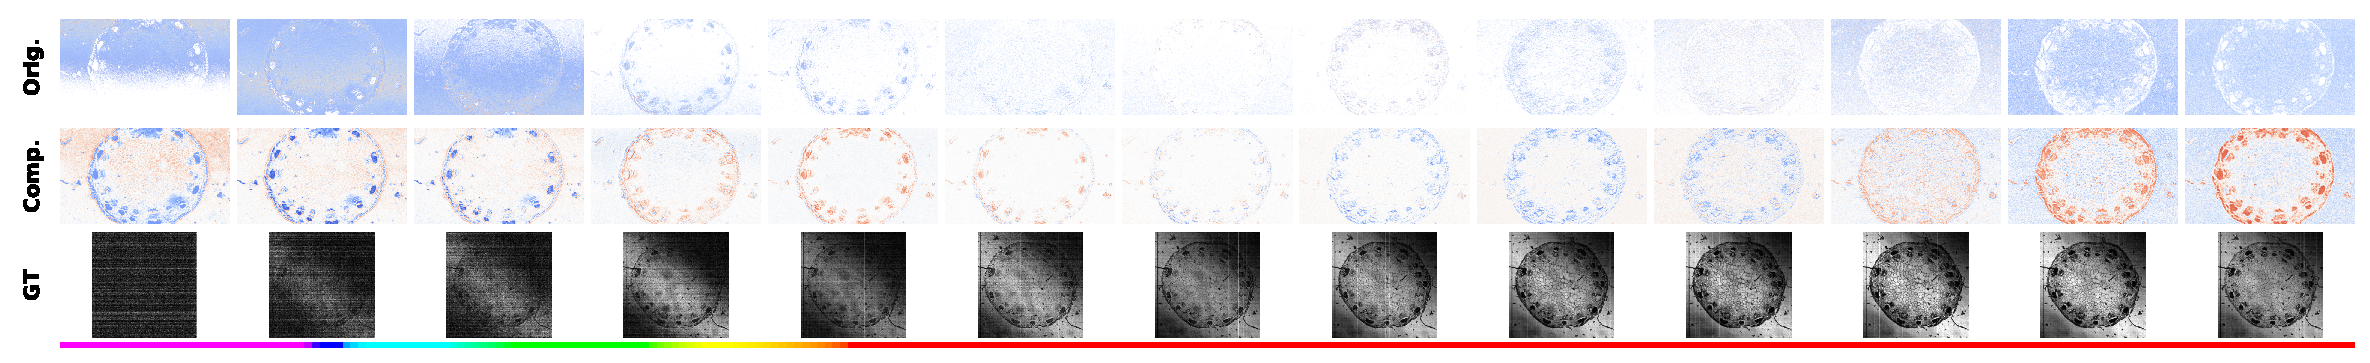
\includegraphics[width=0.98\textwidth]{../../publication_code/figures/figure04_allinone_20251101_161009/figure04_rescaled_grid_bins_03_15.pdf}
% 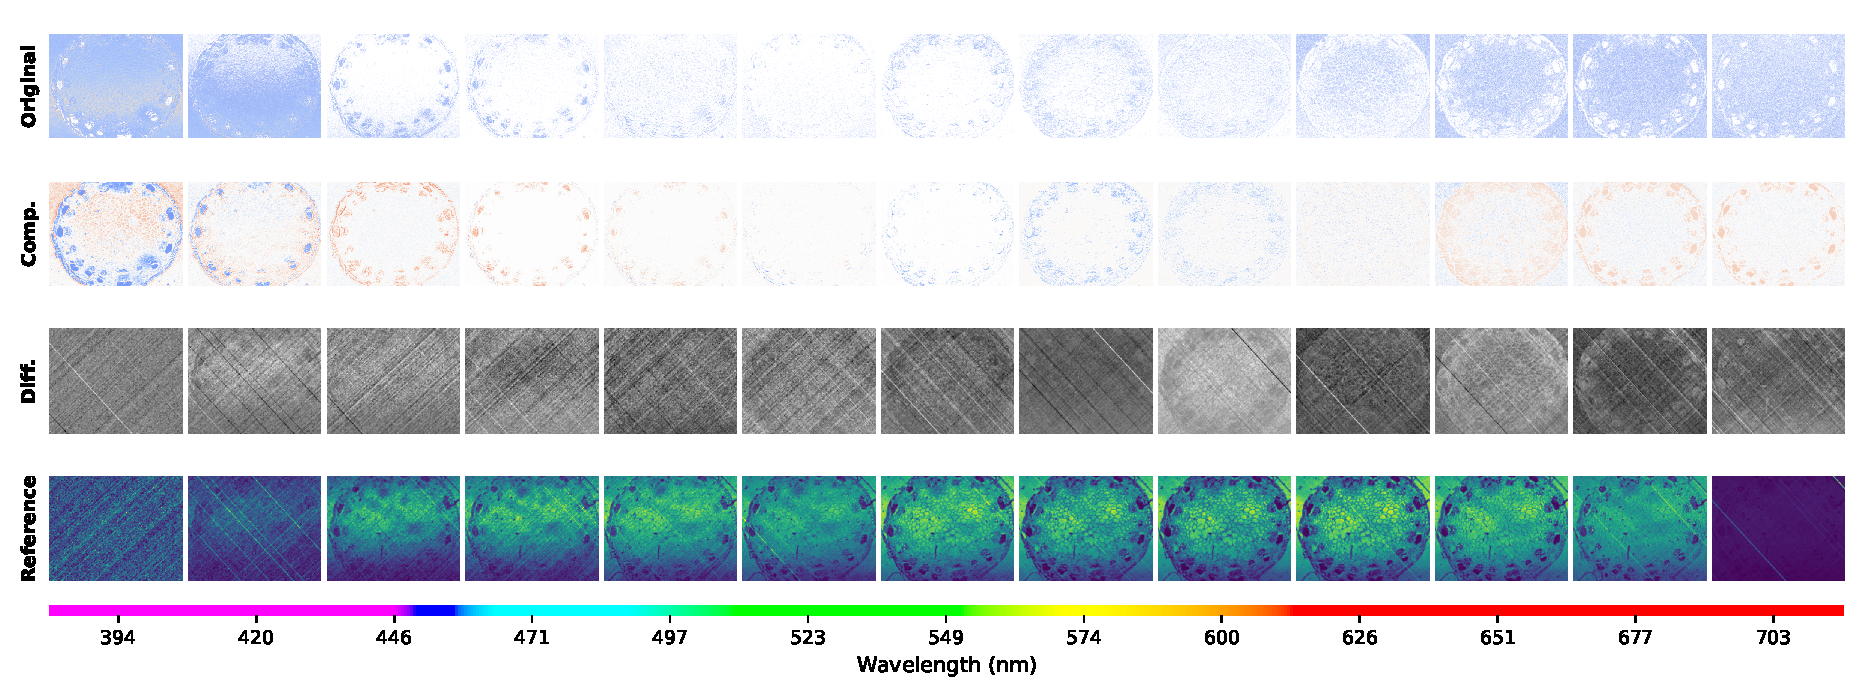
\includegraphics[width=0.98\textwidth]{figures/spectral_reconstruction_scan_rotated_cropped_400_700.pdf}
%   \caption{
%   % Spectral reconstruction across a single forward scan. Each column shows a 50~ms temporal bin.
%    % (top: original; bottom: compensated with 3$\times$3$\times$3 smoothing and background subtraction). 
%    Spectral reconstruction across a single forward scan. The view spans 175--775~ms (\(\approx 390\) to 660~nm). Columns sample five 50~ms bins centred near 389, 456, 523, 590, and 657~nm. Rows (top to bottom): original cumulative events, multi-window compensated accumulation, 20~nm wavelength-gradient slices from the reference hyperspectral camera, and the 300~s reference exposure.
%    }
%   \label{fig:spectrum}
% \end{figure*}

\olsection{System architecture and sensing model}
% Figure~\ref{fig:overview} sketches the optical layout. 
Our system consists of a dispersed illumination module and a detection module (Figure~\ref{fig:overview}). 
% A broadband LED source passes through a slit and diffraction grating before illuminating the specimen.
% The transmitted light is collected by a microscope and relayed through a 4$f$ system onto a hybrid detection plane comprising an event camera and a frame camera. 
% The illumination path uses a broadband LED with a slit and diffraction grating to project different wavelengths cross the specimen, while the detection path uses a 4$f$ relay to feed both an event camera and a frame sensor. 
In the illumination path, a broadband LED with a slit and diffraction grating projects different wavelengths across the specimen. The transmitter light is collected and relayed (4$f$ system) to both an event camera and frame sensor.
This configuration preserves the original microscope imaging via a beam splitter and enables synchronous event and frame capture. 
% The motor executes repeated forward/backward scans, but its speed is neither constant nor calibrated.
The motor repeatedly scans forwrd and backward at an uncalibrated, non-uniform speed. 

Under small-angle assumptions the wavelength incident on pixel $(x,y)$ is
\begin{equation}
  \lambda(x,t) \approx d\!\left(\frac{x}{z_2} - \frac{\xi(t)}{z_1}\right),
  \label{eq:lambda_mapping}
\end{equation}
where $d$ is the grating dispersion constant, $z_2$ and $z_1$ denote distances from the grating to the sensor and illumination relay, and $\xi(t)$ is the motor displacement inferred from the data stream. The transmitted intensity can be written as $I_{x,y}(t) = I_0^{(x,y)}[\lambda(x,t)]$, leading to the temporal gradient
\begin{equation}
  \frac{\partial I_{x,y}}{\partial t} = \frac{\partial I_0^{(x,y)}}{\partial \lambda} \frac{\partial \lambda(x,t)}{\partial t},
  \label{eq:intensity_gradient}
\end{equation}
which drives event emission when the logarithmic intensity crosses the sensor threshold~\cite{yu2025active}. Because $\partial \lambda/\partial t$ is governed by the motor trajectory, reconstructing $I_0^{(x,y)}(\lambda)$ reduces to integrating events along a synchronized wavelength axis.

\begin{figure}[t]
  \centering
  \begin{tikzpicture}
    \node[anchor=south west, inner sep=0] (f2b) at (0,0)
      % {\includegraphics[width=\linewidth]{../../publication_code/figures/figure02_correlation.pdf}};
      {\includegraphics[width=1\linewidth]{figures/figure02_correlation.pdf}};
    \begin{scope}[x={(f2b.south east)}, y={(f2b.north west)}]
      \node[font=\bfseries, anchor=north west, fill=none, text=black, inner sep=2pt] at (-0.05, 1.05) {(a)};
    \end{scope}
  \end{tikzpicture}\\[-0pt]
  % \vspace{-10pt}
  \begin{tikzpicture}
    \node[anchor=south west, inner sep=0] (f2a) at (0,0)
      % {\includegraphics[width=\linewidth]{../../publication_code/figures/figure02_activity.pdf}};
      {\includegraphics[width=1\linewidth]{figures/figure02_activity.pdf}};
    \begin{scope}[x={(f2a.south east)}, y={(f2a.north west)}]
      \node[font=\bfseries, anchor=north west, fill=none, text=black, inner sep=2pt] at (-0.05, 1.05) {(b)};
    \end{scope}
  \end{tikzpicture}\\[-0pt]
  % \vspace{-10pt}
  \caption{Self-synchronized scan segmentation. (a) Auto-correlation and auto-convolution of the event activity signal; the red and blue marker indicates the peak used to determine the period, start and end of scanning. (b) Event counts over the full recording with pre- and post-scan shading and alternating forward and backward boundaries. }
  \label{fig:segmentation}
\end{figure}


\begin{figure}[t]
  \centering
  % \vspace{-20pt}
  % (a) 3D event cloud before compensation
  \begin{tikzpicture}
    \node[anchor=south west, inner sep=0] (img3a) at (0,0)
      {\includegraphics[width=1\linewidth]{figures/event_cloud_before.pdf}};
    \begin{scope}[x={(img3a.south east)}, y={(img3a.north west)}]
      \node[font=\bfseries, anchor=north west, fill=none, text=black, inner sep=2pt]
        at (-0.05, 1.050) {(a)};
      % Discrete polarity legend using node circles (immune to x/y anisotropy)
      \def\lx{0.90}\def\ly{0.97}
      \node[draw=black, fill=evtNeg, circle, minimum size=2mm, inner sep=0pt] at (\lx,\ly) {};
      \node[anchor=west, inner sep=1pt, scale=0.7] at (\lx+0.03, \ly) {$-1$};
      \node[draw=black, fill=evtPos, circle, minimum size=2mm, inner sep=0pt] at (\lx,\ly-0.06) {};
      \node[anchor=west, inner sep=1pt, scale=0.7] at (\lx+0.03, \ly-0.06) {$+1$};
    \end{scope}
  \end{tikzpicture}\\[-10pt]

  % (b) 3D event cloud after compensation
  \begin{tikzpicture}
    \node[anchor=south west, inner sep=0] (img3b) at (0,0)
      {\includegraphics[width=1\linewidth]{figures/event_cloud_after.pdf}};
    \begin{scope}[x={(img3b.south east)}, y={(img3b.north west)}]
      \node[font=\bfseries, anchor=north west, fill=none, text=black, inner sep=2pt]
        at (-0.05, 1.050) {(b)};
    \end{scope}
  \end{tikzpicture}\\[-0pt]

  % (c,d) Plain overlay images (original vs. compensated), side-by-side
  \begin{minipage}[t]{0.49\linewidth}
    \begin{tikzpicture}
      \node[anchor=south west, inner sep=0] (img3c) at (0,0)
        {\includegraphics[width=\linewidth]{figures/overlay_image_before_plain.pdf}};
      \begin{scope}[x={(img3c.south east)}, y={(img3c.north west)}]
        \node[font=\bfseries, anchor=north west, fill=none, text=black, inner sep=2pt]
          at (-0.05, 1.15) {(c)};
      \end{scope}
    \end{tikzpicture}
  \end{minipage}\hfill
  \begin{minipage}[t]{0.49\linewidth}
    \begin{tikzpicture}
      \node[anchor=south west, inner sep=0] (img3d) at (0,0)
        {\includegraphics[width=\linewidth]{figures/overlay_image_after_plain.pdf}};
      \begin{scope}[x={(img3d.south east)}, y={(img3d.north west)}]
        \node[font=\bfseries, anchor=north west, fill=none, text=black, inner sep=2pt]
          at (-0.05, 1.15) {(d)};
        % Continuous color bar (coolwarm-like) inside panel (d)
        \def\xb{1.02}\def\yb{0.10}\def\wb{0.035}\def\hb{0.80}
        \shade[bottom color=evtNeg, top color=white] (\xb,\yb) rectangle (\xb+\wb, \yb+0.5*\hb);
        \shade[bottom color=white, top color=evtPos]  (\xb,\yb+0.5*\hb) rectangle (\xb+\wb, \yb+\hb);
        \node[anchor=west, inner sep=1pt, scale=0.7] at (\xb+\wb+0.01, \yb) {$-1$};
        \node[anchor=west, inner sep=1pt, scale=0.7] at (\xb+\wb+0.01, \yb+0.5*\hb) {$0$};
        \node[anchor=west, inner sep=1pt, scale=0.7] at (\xb+\wb+0.01, \yb+\hb) {$1$};
      \end{scope}
    \end{tikzpicture}
  \end{minipage}\\[-2pt]

  \caption{Multi-window scanning compensation results. Panels (a) and (b) show 3D event clouds before and after compensation, respectively. In each, a dashed outline (red in (a), green in (b)) marks the spatial footprint of a 50~ms temporal accumulation range within the cloud. Panels (c) and (d) show the corresponding normalized event accumulations over this same 50~ms range (before and after compensation).}
  \label{fig:warp}
\end{figure}

\begin{figure}[t]
  \centering
  % Single aligned overlay (Background vs Groundtruth)
  % \includegraphics[width=\columnwidth]{../../publication_code/figures/figure04_allinone_20251103_214813/figure04_rescaled_bg_gt_third_only.png}
  \includegraphics[width=\columnwidth]{figures/figure04_edges_only_third.pdf}\\[-10pt]
  \caption{Aligned background mapped to wavelength using the auto-alignment (\SIrange{400}{700}{\nano\meter} $\approx$ \SIrange{236}{821}{\milli\second} in
  the background timeline) compared against a single spectrometer curve. }
  \label{fig:figure5}
\end{figure}

% \begin{figure*}[t]
%   \centering
%   % 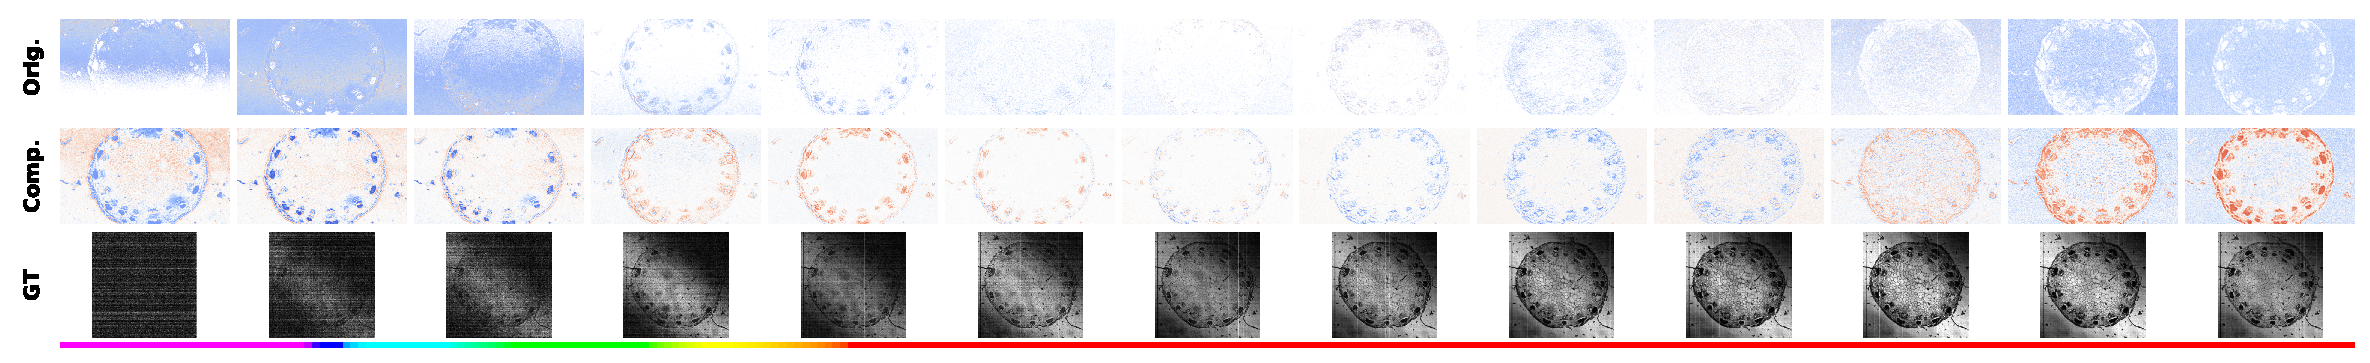
\includegraphics[width=0.98\textwidth]{../../publication_code/figures/figure04_allinone_20251101_161009/figure04_rescaled_grid_bins_03_15.pdf}
% 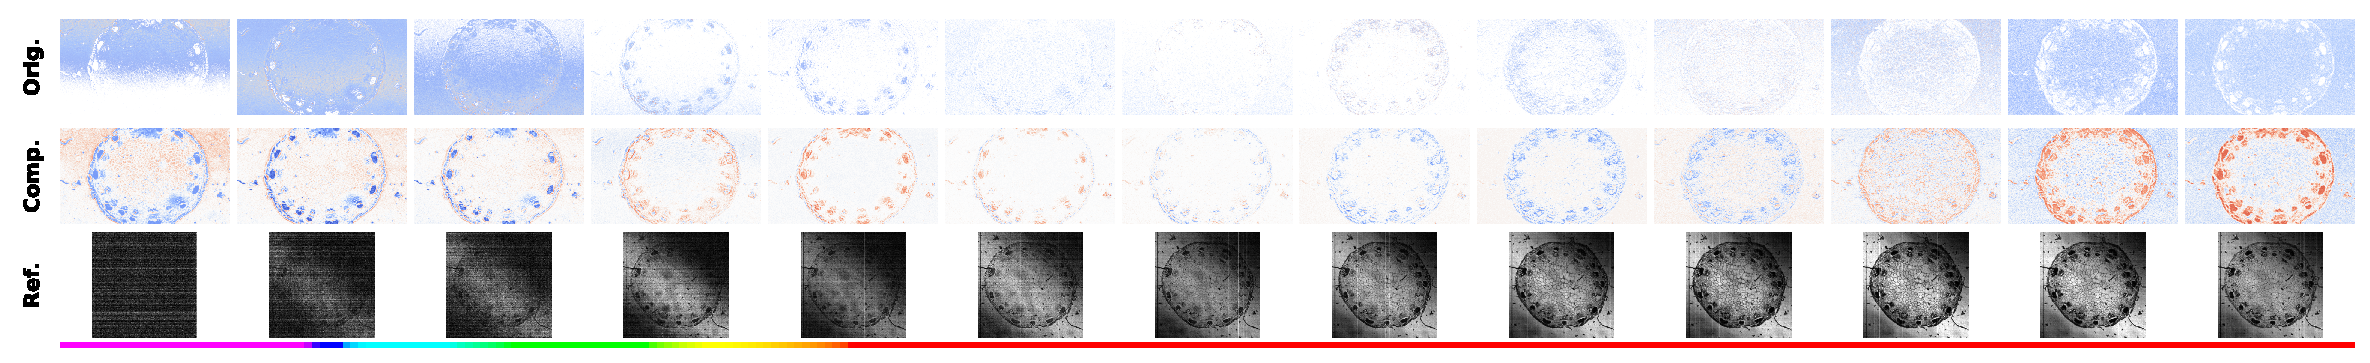
\includegraphics[width=0.98\textwidth]{figures/figure04_rescaled_grid_bins_03_15.pdf}
%   \caption{
%   Spectral reconstruction across a single forward scan. Each column shows a 50~ms temporal bin.
%    % (top: original; bottom: compensated with 3$\times$3$\times$3 smoothing and background subtraction). 
%    }
%   \label{fig:spectrum}
% \end{figure*}



\begin{figure*}[t]
  \centering
  % 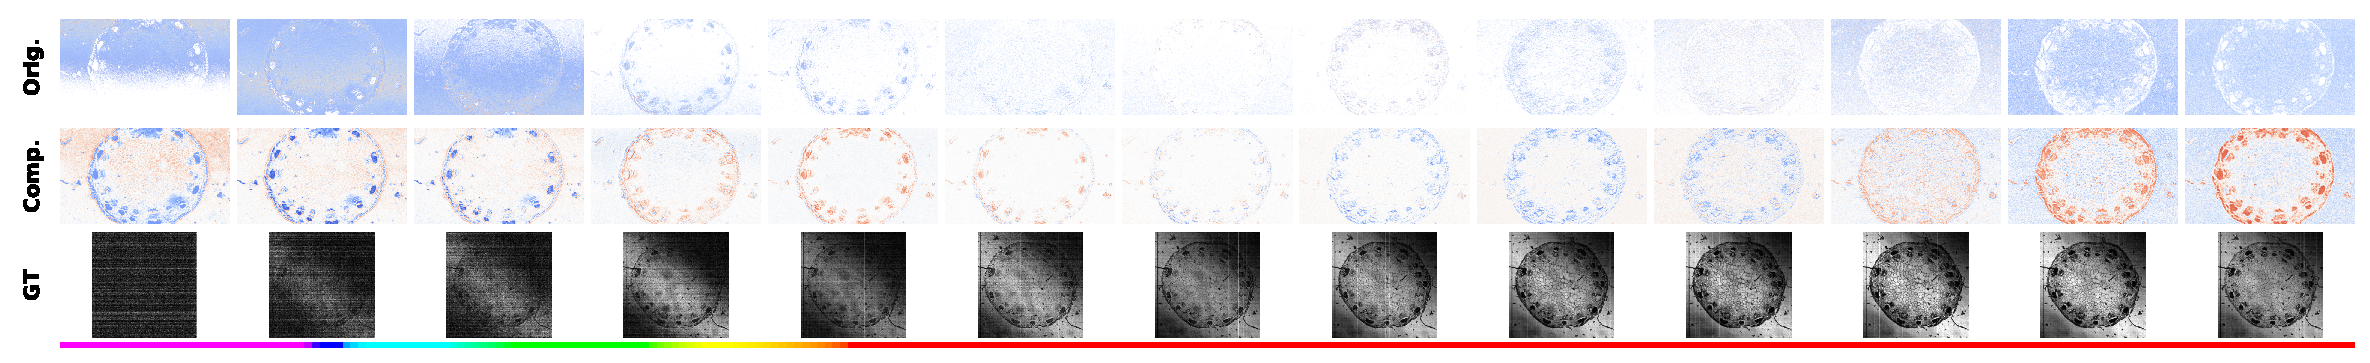
\includegraphics[width=0.98\textwidth]{../../publication_code/figures/figure04_allinone_20251101_161009/figure04_rescaled_grid_bins_03_15.pdf}
  % Wrap in TikZ to overlay a scale bar (full-width of cropped sensor image \approx 2 mm; 50\,\textmu m bar = 2.5\% width)
  \begin{tikzpicture}
    \node[anchor=south west, inner sep=0] (specimg) at (0,0)
      {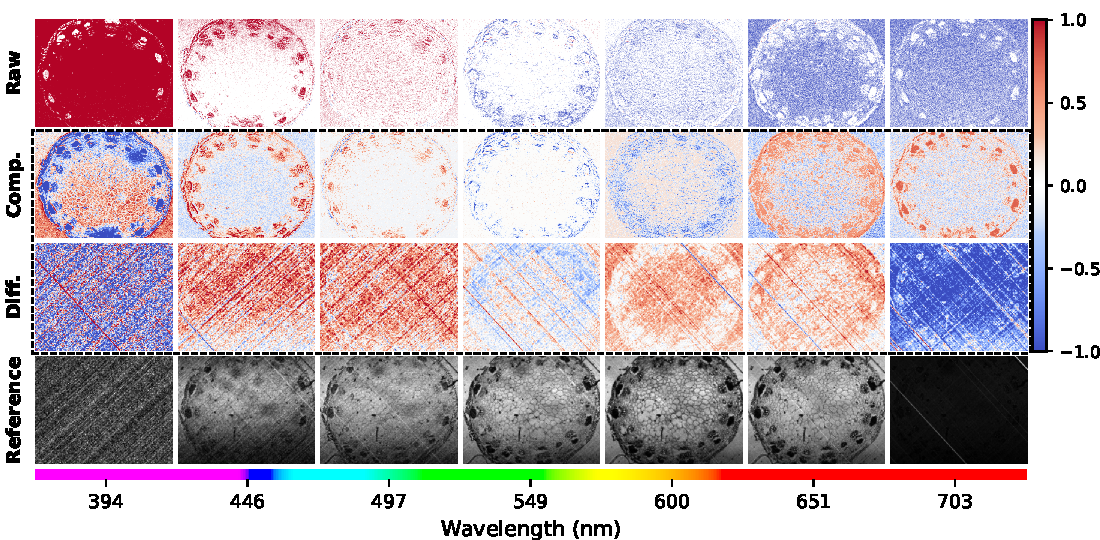
\includegraphics[width=0.98\textwidth]{figures/spectral_reconstruction_scan_rotated_cropped_400_700_wllist_signedraw_q95_sharednorm_fullbar_ticks_labels_v3.pdf}};
    \begin{scope}[x={(specimg.south east)}, y={(specimg.north west)}]
      % Normalized coordinates: (0,0) bottom-left, (1,1) top-right
      % Place a 50\,\textmu m scale bar (2.5% of width) near lower-right
      \def\sx{0.42}\def\sy{0.78}\def\sw{0.025}\def\sh{0.008}
      % Transparent background (no backing pad)
      % Black bar
      \fill[black] (\sx, \sy) rectangle (\sx+\sw, \sy+\sh);
      % Label (black text)
      \node[anchor=west, inner sep=1pt, scale=0.9] at (\sx+\sw+0.01, \sy+0.002) {$300\,\micro\meter$};
    \end{scope}
  \end{tikzpicture}\\[-0pt]
  \caption{
  % Spectral reconstruction across a single forward scan. Each column shows a 50~ms temporal bin.
   % (top: original; bottom: compensated with 3$\times$3$\times$3 smoothing and background subtraction). 
   % Spectral reconstruction across a single forward scan (236--821~ms, $\approx$400--700~nm). Columns sample seven 50~ms bins centred at 394, 446, 497, 549, 600, 651, and 703~nm. All rows share a color scale normalized to the global 95th percentile magnitude within each row. Rows (top to bottom): 50~ms raw event accumulations; 50~ms compensated accumulations; 20~nm finite-difference gradients from the hyperspectral reference stack; and reference exposures from the frame-based hyperspectral camera. The dashed box highlights the compensated and gradient rows, which provide the closest available basis for qualitative comparison with the hyperspectral reference, though they are not pixelwise ground-truth correspondences.
   Spectral reconstruction results(236--821~ms, $\approx$400--700~nm). Columns show seven 50~ms bins from 394 to 703~nm. All rows use a color scale normalized to the global 95th-percentile magnitude within each row. Rows (top to bottom): 50~ms raw event accumulations; 50~ms compensated accumulations; 20~nm finite-difference gradients from the hyperspectral reference; and reference exposures from the frame-based hyperspectral camera. The dashed box highlights the compensated and gradient rows, which provide the closest basis for qualitative comparison with the hyperspectral reference, though not pixelwise ground-truth.
   }
  \label{fig:spectrum}
\end{figure*}

% \olsection{Event-trigger probability model}
% Event emission occurs when the logarithmic brightness increment surpasses a fixed magnitude $\theta$. Under realistic sensing conditions the observed gradient is corrupted by noise, which we model as
% \begin{equation}
%   \nabla I = \nabla I_{\text{true}} + \eta,\qquad \eta \sim \mathcal{N}(0,\sigma^2).
%   \label{eq:gradient_noise}
% \end{equation}

% The probability of a positive event equals the likelihood that the noise-perturbed gradient exceeds the threshold,
% \begin{equation}
%   P(\text{event}) = P(\eta > \theta - \nabla I_{\text{true}}) = \tfrac12\!\left[1 - \operatorname{erf}\!\left(\frac{\theta - \nabla I_{\text{true}}}{\sqrt{2}\sigma}\right)\right],
%   \label{eq:trigger_probability}
% \end{equation}
% with an analogous form for negative events around $-\theta$. Approximating the error function by a logistic curve yields the computationally convenient sigmoid expression
% \begin{equation}
%   P(\text{event}) \approx \sigma\!\left(\frac{\nabla I_{\text{true}} - \theta}{\sigma'}\right),\qquad \sigma' \approx \frac{2\sqrt{2}}{\sqrt{\pi}}\sigma,
%   \label{eq:sigmoid_probability}
% \end{equation}
% where $\sigma(\cdot)$ denotes the logistic sigmoid. Within a temporal bin of duration $\Delta t$ the expected event count relates directly to this probability,
% \begin{equation}
%   \langle N_{\text{evt}}\rangle = \lambda\,P(\text{event})\,\Delta t,
%   \label{eq:expected_events}
% \end{equation}
% with $\lambda$ the effective sampling rate per pixel. Averaging events over repeated scans gives the empirical mean $\bar{N}_{\text{evt}}$, which can be inverted via the logit function $\sigma^{-1}$ to estimate the true gradient:
% \begin{equation}
%   \nabla I_{\text{est}} = \theta + \sigma'\,\sigma^{-1}\!\left(\frac{\bar{N}_{\text{evt}}}{\lambda\,\Delta t}\right).
%   \label{eq:gradient_estimate}
% \end{equation}

% This probabilistic link between event statistics and intensity gradients underpins our reconstruction strategy. Equation~(\ref{eq:gradient_estimate}) justifies using temporally binned events as sufficient statistics for spectral estimation: the scan-induced evolution of $\nabla I_{\text{true}}$ encodes spectral slopes, while averaging suppresses sensor noise and preserves the dynamic-range benefits of event vision. The next section leverage these statistics to segment scans and correct the residual temporal shear before building the spectral cube.

\olsection{Self-synchronized scan segmentation}
% We first convert the event timestamps into an activity signal $a[n]$ (the number of events per 1~ms bin). The peak of auto-correlation
% \begin{equation}
%   R[k] = \sum_{n} a[n]\,a[n+k]
% \end{equation}
% reveals the scanning period, while the auto-convolution of $a[n]$ the correlation of $a[n]$ and its time-reversed sequence $a_{\mathrm{rev}}[n] = a[N{-}1{-}n]$,
% \begin{equation}
%   R_{\mathrm{rev}}[k] = \sum_{n} a[n]\,a[N{-}1{-}n],
%   \label{eq:rev_corr}
% \end{equation}
% exposes the pre- and post-scan regions through the mirror-symmetric peaks around the turnaround time. An iterative peak search refines the start and end indices of each half-scan, producing scanning segments without reference measurements. 
% Event timestamps are binned (1~ms) into an activity trace. 
We first bin event timestamps into a 1~ms activity trace. 
% Two correlation peaks anchor the segmentation: the symmetric auto-correlation peak gives the round-trip period, and the strongest reverse-correlation peak fixes the symmetric turnaround, which jointly set the pre-scan, main scan, and post-scan spans
The auto-correlation of the of this activity exhibits symmetric peaks corresponding to the scan's period. Together with the correlation of the trace with its time-reversed copy (auto-convolution), the start, the turnaround and end of the scan can be retreived without any external timing signals (see \textbf{Supplement 1} for details)~\cite{azevedo2022event}. 
% A brief iterative refinement repeats the peak search after updating these spans, stabilising the forward/backward boundaries without external triggers 
% Figure~\ref{fig:segmentation} illustrates the auto-correlation and auto-convolution used to estimate the scan period, as well as the resulting segmentation of forward and backward passes over the full recording. 
% To verify our self-synchronization approach, we analyzed the event activity over time. 
Figure~2(a) illustrates the auto-correlation of the 1~ms event activity trace, which reveals mirrored peaks at the scan period. The correlation with the reversed signal shows a clear dominant peak including the information of start and end the scanning.
% Figure~\ref{fig:segmentation}(a) shows the auto-correlation of the event count signal along with the auto-convolution correlation with its time-reversed signal. The symmetric peak of the auto-correlation reveals the scanning period and the dominant auto-convolution peak identifies the start and end scanning. 
% The data stream is segmented into forward and backward passes.
Using these peaks, we segment the data stream into forward and backward passes, as visualized in Figure~\ref{fig:segmentation}(b) over the full recording. 
% Figure~\ref{fig:segmentation}(b) visualizes the resulting segmentation over the full recording. 
This data-driven segmentation adapts to slow drifts or perturbations, ensuring that subsequent reconstructions operate on consistent temporal support. 
% Planned figs include (i) using only the first forward/back pair to quantify baseline noise, and (ii) averaging all three pairs to demonstrate variance reduction. 

\olsection{Multi-window scanning compensation}
Even with accurate segmentation, residual non-uniform motor motion introduces spatially varying temporal delays and shear in the event cloud. We therefore model each scan as a sequence of $M$ temporal windows, each with its own local affine time warp whose slopes vary smoothly across the field (full parameterization in \textbf{Supplement~1}); here we summarize the optimization.
% Even with accurate segmentation, \eqref{eq:lambda_mapping} introduces a spatially varying delay through the $x/z_2$ term; motor acceleration near turnarounds further shears the time axis. Our multi-window compensation routine addresses this by fitting boundary surfaces
% \begin{equation}
%   T_i(x,y) = a_i x + b_i y + c_i,
% \end{equation}
% which partition each scan into $M$ temporal windows. Soft memberships,
% \begin{equation}
%   w_i(x,y,t) = \frac{\sigma\!\left(\frac{t - T_i}{\tau}\right)\sigma\!\left(\frac{T_{i+1}-t}{\tau}\right)}{\sum_j \sigma\!\left(\frac{t - T_j}{\tau}\right)\sigma\!\left(\frac{T_{j+1}-t}{\tau}\right)},
% \end{equation}
% blend adjacent windows (temperature $\tau \approx 1$~ms). The compensated time is
% \begin{equation}
%   t' = t - \sum_{i=1}^{M-1} w_i(x,y,t)\bigl(\tilde{a}_i x + \tilde{b}_i y \bigr),
%   \label{eq:timewarp}
% \end{equation}
% where $\{\tilde{a}_i,\tilde{b}_i\}$ are trainable slopes optimized by minimizing the spatial variance of binned event intensities while enforcing smoothness across neighbouring windows. The objective is 
% \begin{equation}
% \begin{split}
%   \mathcal{L}(\theta)
%   &= 
%   \underbrace{
%   \tfrac{1}{HW}\!\sum_k\!\sum_{x,y}
%   \bigl(\mathsf{E}_k(x,y;\theta)-\mu_k\bigr)^2
%   }_{\mathcal{L}_{\mathrm{var}}} \\[3pt]
%   &\quad + 
%   \lambda_{\mathrm{sm}}
%   \underbrace{
%   \sum_{i=1}^{M-2}
%   \!\Big[
%   (\tilde{a}_{i+1}-\tilde{a}_i)^2
%   +(\tilde{b}_{i+1}-\tilde{b}_i)^2
%   \Big]
%   }_{\mathcal{L}_{\mathrm{sm}}},
%   \label{eq:loss}
% \end{split}
% \end{equation}
% where $\mathsf{E}_k(x,y)$ is the compensated event frame in bin $k$, $\mu_k = (HW)^{-1}\sum_{x,y}\mathsf{E}_k(x,y)$ is its spatial mean, and $\lambda_{\mathrm{sm}}$ controls the smoothness strength. Minimizing $\mathcal{L}(\theta)$ by gradient descent aligns temporal windows, suppresses acceleration-induced shear, and yields sharper spectral reconstructions than a single-plane warp.

Given a set of warp parameters $\theta$ (collecting all learned slopes and offsets), the raw events are mapped from their original timestamps $t$ to compensated times $t'(x,y,t;\theta)$, and then accumulated into frames $\mathsf{E}_k(x,y;\theta)$ for each temporal bin $k$. We choose $\theta$ by minimizing
\begin{equation}
\begin{split}
  \mathcal{L}(\theta)
  &= 
  \underbrace{
  \tfrac{1}{HW}\!\sum_k\!\sum_{x,y}
  \bigl(\mathsf{E}_k(x,y;\theta)-\mu_k\bigr)^2
  }_{\mathcal{L}_{\mathrm{var}}} \\[3pt]
  &\quad + 
  \lambda_{\mathrm{sm}}
  \underbrace{
  \sum_{i=1}^{M-2}
  \!\Big[
  (\tilde{a}_{i+1}-\tilde{a}_i)^2
  +(\tilde{b}_{i+1}-\tilde{b}_i)^2
  \Big]
  }_{\mathcal{L}_{\mathrm{sm}}},
  \label{eq:loss}
\end{split}
\end{equation}
where $H$ and $W$ are the image height and width, $\mathsf{E}_k(x,y;\theta)$ is the compensated event frame in bin $k$, and $\mu_k = (HW)^{-1}\sum_{x,y}\mathsf{E}_k(x,y;\theta)$ is its spatial mean. The coefficients $\tilde{a}_i$ and $\tilde{b}_i$ denote the effective lateral and vertical time-per-pixel slopes in window $i$, and $\lambda_{\mathrm{sm}}$ controls the strength of the smoothness penalty that encourages neighbouring windows to have similar slopes. The variance term $\mathcal{L}_{\mathrm{var}}$ favours sharp, spatially coherent accumulations within each temporal bin, while the regularizer $\mathcal{L}_{\mathrm{sm}}$ prevents overfitting by enforcing a slowly varying time-warp across windows. Minimizing $\mathcal{L}(\theta)$ by gradient descent aligns the temporal windows, suppresses acceleration-induced shear, and yields sharper spectral reconstructions than a single-plane warp.


Figure~\ref{fig:warp} summarizes the effects of the proposed multi-window compensation of one scanning segment for a representative specimen (a cross-section of a dicot stem). 
% Panel~(a) illustrates how the learned boundary surfaces align the event distribution in both spatial–temporal projections, effectively capturing the nonuniform scanning motion. 
% The fitted slopes span from  \SI{-1.74}{\micro\second\per\pixel} to \SI{5.50}{\micro\second\per\pixel} for \(X\)-axis, and from \SI{-79.82}{\micro\second\per\pixel} to \SI{-75.67}{\micro\second\per\pixel} for \(Y\)-axis, representing the lateral and vertical time-per-pixel coefficients of the multi-window model.
% Panel~(b) shows that the temporal variance within each 50~ms bin decreases after compensation, indicating improved temporal coherence across the field of view. 
% Panel~(c) compares representative cumulative event frames before and after correction, where the removal of diagonal blur patterns confirms that the time-warp model successfully restores the spatial integrity of each spectral slice.
Panels~\ref{fig:warp}(a) and \ref{fig:warp}(b) show 3D event clouds before and after applying the learned time-warp, highlighting the removal of the spatial–temporal shear caused by motor motion. In each panel, a dashed box marks the spatial extent of a short (50~ms) accumulation range used for comparison. 
Panels~\ref{fig:warp}(c) and \ref{fig:warp}(d) present the corresponding event accumulations  before and after the compensation over the same temporal range. Together these panels demonstrate that the multi-window model effectively corrects motion-induced distortions across the view.

\olsection{Time--wavelength auto-alignment}
% A one-dimensional background trace $b(t)$ is first computed from polarity-weighted, compensated events using a fixed step of 5~ms. After normalising this trace between its pre- and post-scan plateaus, the active scanning interval $[t_0,t_1]$ is identified from the rising and falling edges of the smoothed signal. This provides a robust estimate of when the illumination enters and leaves the sample.
We first compute a one-dimensional background trace $b(t)$ by integrating polarity-weighted events in 5~ms bins. After normalizing $b(t)$ between its pre- and post-scan plateaus, we locate the active scan interval $[t_0, t_1]$ from where the trace rises and falls—indicating when illumination enters and exits the sample.

% For each reference spectrum $g_i(\lambda)$ with known wavelength support, the corresponding time interval is fitted with a simple affine model $\lambda(t)=\alpha t+\beta$, where the slope and intercept are obtained from the average boundary wavelengths across all calibration curves. 
For each reference spectrum $g_i(\lambda)$ (with known wavelength endpoints), we fit a simple affine model $\lambda(t) = \alpha t + \beta$ over its corresponding time interval. We determine $\alpha$ and $\beta$ from the average start- and end-wavelengths across all calibration curves.
The normalised background trace is then reparameterised from time to wavelength using this mapping and matched to the mean ground-truth spectrum via a least-squares fit for amplitude.

This calibrated time--wavelength mapping underpins the spectral sequence in Fig.~\ref{fig:spectrum}, where reconstructed slices are indexed directly by wavelength. 
Figure~\ref{fig:figure5} shows the background alignment result, where the event-derived wavelength mapping agrees closely with the spectrometer reference curve.



\olsection{Spectral reconstruction and benchmarking}
After compensation, events are cumulated along $t'$ into quasi-static frames $\mathsf{E}_k(x,y)$, with each cumulative window advanced by a \SI{5}{\milli\second} temporal step, and polarity-weighted counts integrated to recover relative spectra. 
% Figure~\ref{fig:spectrum} illustrates the reconstructed spectral sequence across a single forward scan, showing the temporal evolution of wavelength-dependent features derived from the event stream.
With the temporal alignment and wavelength calibration in place, we reconstruct the spectral sequence. 
Figure~\ref{fig:spectrum} compares our event-based reconstruction with the output of a conventional hyperspectral camera. The top two rows show 50~ms event accumulations before and after multi-window compensation; the third row displays the corresponding 20~nm finite-difference gradients derived from the reference hyperspectral stack; and the bottom row provides the camera’s raw intensity images for those wavelengths. 
As highlighted by the dashed box, the compensated event-based slices most closely resemble the reference gradients, demonstrating that the proposed pipeline captures wavelength-dependent structure.
Table~\ref{tab:acquisition_comparison} summarizes the acquisition time and cost differences between the proposed event-driven system and a conventional frame-based hyperspectral camera. 
Under the same illumination condition, our event-driven system completes a full spectral scan within \SIrange{150}{1100}{\milli\second}, whereas the reference hyperspectral camera requires approximately \SI{300}{\second} for an equivalent acquisition. The event-driven acquisition also reduces data volume by nearly an order of magnitude (18.5~MB versus 138~MB), enabling faster data transfer and lighter storage requirements, which are advantageous for portable or embedded implementations.
All structural components of our prototype are 3D printed using an Ultimaker~3S printer, while the optical and mechanical parts include a standard 2835 surface-mount LED under \SI{1}{\USD}, a diffraction grating priced at about \SI{1.3}{\USD} and a motor–controller set costing approximately \SI{32.5}{\USD}. The total material cost of the complete event hyperspectral system is therefore below \SI{35}{\USD}. 
In addition to the drastic reduction in acquisition time and cost, the asynchronous sensing architecture offers high dynamic range and resilience to illumination fluctuations, maintaining reliable performance even in low-light environments where the frame-based camera exhibits noise saturation and motion blur. 
These results highlight the efficiency and practicality of self-synchronized, event-based hyperspectral imaging for compact and adaptive optical platforms.

\begin{table}[t]
\centering
\caption{Acquisition time and cost comparison between the proposed event-driven system and a reference hyperspectral camera.}
\label{tab:acquisition_comparison}
\begin{tabular}{lcc}
\hline
\textbf{Parameter} & \textbf{Ours} & \textbf{Reference camera} \\
\hline
Acquisition time & $\sim$\SI{585}{\milli\second} per scan & \SI{300}{\second} per scan \\
Data volume & \SI{18.5}{\mega\byte} & \SI{138}{\mega\byte} \\
Approx.\ price & $\sim$\SI{3000}{\USD} & \SI{14000}{\USD} \\
\hline
\end{tabular}
\end{table}

\olsection{Discussion and outlook}
% The self-synchronizing strategy removes the need for encoder calibration while tolerating speed fluctuations from cost-effective actuators, distinguishing this platform from prior systems that assumed precise timing hardware
Our self-synchronizing strategy removes the need for encoder calibration and tolerates speed fluctuations from low-cost actuators. This capability distinguishes our platform from prior systems that required precision timing hardware
~\cite{hagen2013review,yeh2011selfcal}. Our variance-minimizing, multi-window time warp builds upon piecewise-affine compensations used in event-based motion estimation~\cite{mitrokhin2018mobility}, adapting them to the spectral scanning context. Together these components enable transmission-mode spectral capture without illumination modulation or auxiliary sensors.

% Planned figures: (i) gather datasets spanning single and triple scan fusion to populate Fig.~\ref{fig:segmentation}(d); (ii) quantify variance reduction and residual blur for multi-window versus single-plane warps to complete Fig.~\ref{fig:warp}; and (iii) collect spectral overlays under nominal and low-light scenarios to fill Fig.~\ref{fig:spectrum}. 

\olsection{Conclusion}
% We present a self-synchronized, event-driven transmission hyperspectral system that derives scan timing from the event stream and compensates temporal shear using a multi-window time warp. 
We demonstrate a self-synchronized, event-driven transmission hyperspectral system that derives its scan timing from the event data and uses a multi-window time warp to correct temporal shear.
Despite relying on inexpensive, non-uniform motor motion, the reconstructed spectra align with a reference hyperspectral camera and retain fidelity under reduced illumination. 

\begin{backmatter}
\bmsection{Funding}
The work was supported by the Research Grants Council of Hong Kong (GRF 17201822 and RIF R7003-21).

% \bmsection{Acknowledgment}

\bmsection{Disclosures}
The authors declare no conflicts of interest.

\bmsection{Data Availability}
Data underlying the results presented in this paper are available from the corresponding author upon reasonable request. All 3D-printable components, design files, and source code used in this work are openly accessible at the provided GitHub repository.

\bmsection{Supplemental document}
See \textbf{Supplement 1} for supporting content.
\end{backmatter}

\bibliography{ref}

\end{document}
